\begin{name}
	{\tenchude}{\tendethi}{LỚP TOÁN THẦY PHÁT}{\thoigian}
\end{name}
 
\setcounter{ex}{0}\setcounter{bt}{0}
\Opensolutionfile{ans}[ans/ans-2-TT-23-SoGDDT-BinhPhuoc-23]
\begin{ex}%[Đề thi thử Tốt Nghiệp THPT Lần 1, SGD Bình Phước, 2023]%[12-EX-6-2023, Võ Hoàng Nghĩa]%[2D2Y4-2]
	Trên khoảng $(0;+\infty)$, đạo hàm của hàm số $y=\log_5x$ là
	\choice
	{\True $y'=\dfrac{1}{x\ln 5}$}
	{$y'=x\ln 5$}
	{$y'=\dfrac{\ln 5}{x}$}
	{$y'=\dfrac{x}{\ln 5}$}
	\loigiai{
		Ta có $\left(\log_5x\right)'=\dfrac{1}{x\ln 5}$.
	}
\end{ex}

\begin{ex}%[Đề thi thử Tốt Nghiệp THPT Lần 1, SGD Bình Phước, 2023]%[12-EX-6-2023, Võ Hoàng Nghĩa]%[2D2Y6-1]
	Tập nghiệm của bất phương trình $\log x<1$ là
	\choice
	{$(-\infty;1)$}
	{$(10;+\infty)$}
	{$(-\infty;10)$}
	{\True $(0;10)$}
	\loigiai{
		Ta có $\log x<1\Leftrightarrow\heva{
			&x>0\\ 
			&x<10\\}\Leftrightarrow 0<x<10$.\\
		Vậy tập nghiệm của bất phương trình là $S=(0;10)$.
	}
\end{ex}

\begin{ex}%[Đề thi thử Tốt Nghiệp THPT Lần 1, SGD Bình Phước, 2023]%[12-EX-6-2023, Võ Hoàng Nghĩa]%[2D1Y2-2]
	Cho hàm số $y=f(x)$ có bảng biến thiên như hình vẽ sau
	\begin{center}
		
\begin{tikzpicture}
			\tkzTabInit[lgt=1,espcl=2]{$x$/0.6,$y'$/0.6,$y$/2}{$-\infty$,$-2$,$0$,$2$,$+\infty$}  
			\tkzTabLine{,+,0,-,0,+,0,-,}
			\tkzTabVar{-/$-\infty$,+/$3$,-/$-1$,+/$3$,-/$-\infty$}  
		\end{tikzpicture}
	\end{center}
	Giá trị cực đại của hàm số đã cho bằng
	\choice
	{$2$}
	{\True $3$}
	{$-2$}
	{$-1$}
	\loigiai{
		Từ bảng biến thiên, ta thấy giá trị cực đại của hàm số đã cho bằng $3$.
	}
\end{ex}

\begin{ex}%[Đề thi thử Tốt Nghiệp THPT Lần 1, SGD Bình Phước, 2023]%[12-EX-6-2023, Võ Hoàng Nghĩa]%[2D2Y6-2]
	Tập nghiệm của bất phương trình $\left(\dfrac{1}{2}\right)^x>8$ là
	\choice
	{$(-\infty ;3)$}
	{\True $(-\infty ;-3)$}
	{$(3;+\infty)$}
	{$(-3;+\infty)$}
	\loigiai{
		Ta có $\left(\dfrac{1}{2}\right)^x>8\Leftrightarrow 2^{-x}>2^3 \Leftrightarrow -x>3 \Leftrightarrow x<-3$.\\
		Vậy bất phương trình có tập nghiệm là $S=(-\infty ;-3)$.
	}
\end{ex}

\begin{ex}%[Đề thi thử Tốt Nghiệp THPT Lần 1, SGD Bình Phước, 2023]%[12-EX-6-2023, Võ Hoàng Nghĩa]%[1D3Y4-2]
	Cho cấp số nhân $\left(u_n\right)$ có $u_1=\dfrac{1}{2}$, $u_2=2$. Tìm công bội của cấp số nhân.
	\choice
	{$\dfrac{3}{2}$}
	{$2$}
	{\True $4$}
	{$\dfrac{1}{2}$}
	\loigiai{
		Ta có công bội của cấp số nhân $q=\dfrac{u_2}{u_1}=4$.
	}
\end{ex}

\begin{ex}%[Đề thi thử Tốt Nghiệp THPT Lần 1, SGD Bình Phước, 2023]%[12-EX-6-2023, Võ Hoàng Nghĩa]%[1D2Y2-1]
	Cho tập $S$ có $5$ phần tử. Số tập con gồm đúng $2$ phần tử của $S$ là
	\choice
	{$30$}
	{$5^2$}
	{\True $\mathrm{C}_5^2$}
	{$\mathrm{A}_5^2$}
	\loigiai{
		Số tập con gồm đúng $2$ phần tử của $S$ là $\mathrm{C}_5^2$.
	}
\end{ex}

\begin{ex}%[Đề thi thử Tốt Nghiệp THPT Lần 1, SGD Bình Phước, 2023]%[12-EX-6-2023, Võ Hoàng Nghĩa]%[2D2Y2-2]
	Trên khoảng $(0;+\infty)$, đạo hàm của hàm số $y=x^{\sqrt{2}}$ là
	\choice
	{\True $y'=\sqrt{2}x^{\sqrt{2}-1}$}
	{$y'=\sqrt{2}x^{\sqrt{2}}$}
	{$y'=x^{\sqrt{2}-1}$}
	{$y'=\dfrac{1}{\sqrt{2}}x^{\sqrt{2}-1}$}
	\loigiai{
		Ta có $y'=\sqrt{2}x^{\sqrt{2}-1}$.
	}
\end{ex}

\begin{ex}%[Đề thi thử Tốt Nghiệp THPT Lần 1, SGD Bình Phước, 2023]%[12-EX-6-2023, Võ Hoàng Nghĩa]%[2H3Y1-3]
	Trong không gian $Oxyz$, cho hai điểm $A\left(-3;1;-4\right)$ và $B\left(1;-1;2\right)$. Mặt cầu $(S)$ nhận $AB$ làm đường kính có phương trình là
	\choice
	{$\left(x-4\right)^2+\left(y+2\right)^2+\left(z-6\right)^2=14$}
	{$\left(x-1\right)^2+y^2+\left(z-1\right)^2=14$}
	{$\left(x+1\right)^2+y^2+\left(z+1\right)^2=56$}
	{\True $\left(x+1\right)^2+y^2+\left(z+1\right)^2=14$}
	\loigiai{
		Gọi $I$ là trung điểm đoạn $AB \Rightarrow I (-1;0;-1)$.\\
		Mặt cầu cần tìm có tâm $I\left(-1;0;-1\right)$ và bán kính xác định bởi $$R=IA=\sqrt{\left(-1+3\right)^2+\left(0-1\right)^2+\left(-1+4\right)^2}=\sqrt{14}.$$
		Phương trình của mặt cầu $(S)$ cần tìm là $(x+1)^2+y^2+(z+1)^2=14$.
	}
\end{ex}

\begin{ex}%[Đề thi thử Tốt Nghiệp THPT Lần 1, SGD Bình Phước, 2023]%[12-EX-6-2023, Võ Hoàng Nghĩa]%[2D3Y1-1]
	Họ nguyên hàm của hàm số $f(x)=x-\dfrac{2}{x}$ là
	\choice
	{$\dfrac{x^2}{2}-2\ln x+C$}
	{$\dfrac{x^2}{2}+x+C$}
	{$1+\dfrac{2}{x^2}+C$}
	{\True $\dfrac{x^2}{2}-2\ln\left|x\right|+C$}
	\loigiai{
		Ta có $\displaystyle\int f(x) \mathrm{\,d}x=\int \left(x-\dfrac{2}{x}\right) \mathrm{\,d}x=\dfrac{x^2}{2}-2\ln\left| x\right|+C$.
	}
\end{ex}

\begin{ex}%[Đề thi thử Tốt Nghiệp THPT Lần 1, SGD Bình Phước, 2023]%[12-EX-6-2023, Võ Hoàng Nghĩa]%[2H1Y3-2]
	Cho khối lăng trụ có diện tích đáy bằng $24$, chiều cao bằng $8$. Thể tích của khối lăng trụ đã cho bằng
	\choice
	{\True $192$}
	{$96$}
	{$576$}
	{$64$}
	\loigiai{
		Thể tích của khối lăng trụ bằng $V=Bh=24\cdot 8=192$.
	}
\end{ex}

\begin{ex}%[Đề thi thử Tốt Nghiệp THPT Lần 1, SGD Bình Phước, 2023]%[12-EX-6-2023, Võ Hoàng Nghĩa]%[2D4Y2-2]
	Cho hai số phức $z_1=2+i$ và $z_2=1+3i$. Phần thực của số phức $z_1+z_2$ bằng
	\choice
	{$1$}
	{\True $3$}
	{$4$}
	{$-2$}
	\loigiai{
		Ta có $z_1+z_2=3+4i$.\\
		Phần thực của số phức $z_1+z_2$ bằng $3$.
	}
\end{ex}

\begin{ex}%[Đề thi thử Tốt Nghiệp THPT Lần 1, SGD Bình Phước, 2023]%[12-EX-6-2023, Võ Hoàng Nghĩa]%[2H3Y1-1]
	Trong không gian $Oxyz$, cho véc-tơ $\overrightarrow{a}$ thỏa mãn $\overrightarrow{a}=2\overrightarrow{i}+\overrightarrow{k}-3\overrightarrow{j}$. Tọa độ của véc-tơ $\overrightarrow{a}$ là
	\choice
	{\True $\left(2;-3;1\right)$}
	{$\left(1;2;-3\right)$}
	{$\left(1;-3;2\right)$}
	{$\left(2;1;-3\right)$}
	\loigiai{
		Ta có $\overrightarrow{i}=(1;0;0)$, $\overrightarrow{j}=(0;1;0)$, $\overrightarrow{k}=(0;0;1)$.\\ 
		Do đó $\overrightarrow{a}=(2;-3;1)$.
	}
\end{ex}

\begin{ex}%[Đề thi thử Tốt Nghiệp THPT Lần 1, SGD Bình Phước, 2023]%[12-EX-6-2023, Võ Hoàng Nghĩa]%[2H2Y1-2]
	Cho hình nón có bán kính đáy $R=3$ và độ dài đường sinh $\ell=5$. Diện tích xung quanh của hình nón bằng
	\choice
	{$20\pi$}
	{\True $15\pi$}
	{$25\pi$}
	{$12\pi$}
	\loigiai{
		Diện tích xung quanh của hình trụ là $S_{\text{xq}}=\pi R\ell=\pi\cdot 3\cdot 5=15\pi$.
	}
\end{ex}

\begin{ex}%[Đề thi thử Tốt Nghiệp THPT Lần 1, SGD Bình Phước, 2023]%[12-EX-6-2023, Võ Hoàng Nghĩa]%[2D3Y2-1]
	Nếu $\displaystyle\int\limits_0^2f(x)\mathrm{\,d}x=2$ thì $\displaystyle\int\limits_0^2\left[3f(x)-2\right]\mathrm{\,d}x$ bằng
	\choice
	{$6$}
	{\True $2$}
	{$8$}
	{$4$}
	\loigiai{
		Ta có $\displaystyle\int\limits_0^2\left[3f(x)-2\right]\mathrm{\,d}x=3\int\limits_0^2f(x)\mathrm{\,d}x-2\int\limits_0^2\mathrm{\,d}x=3\cdot2- 2x\Big|_0^2=6-4=2$.
	}
\end{ex}

\begin{ex}%[Đề thi thử Tốt Nghiệp THPT Lần 1, SGD Bình Phước, 2023]%[12-EX-6-2023, Võ Hoàng Nghĩa]%[2D1Y5-1]
	\immini
	{Đồ thị của hàm số nào dưới đây có dạng như đường cong trong hình bên?
		\choice
		{$y=3x^4-2x^2$}
		{\True $y=-x^3+3x$}
		{$y=-x^4+3x^2$}
		{$y=x^3-3x$}}
	{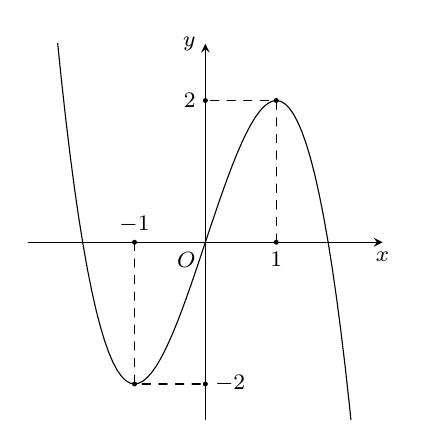
\begin{tikzpicture}[font=\footnotesize,line join=round,line cap=round,>=stealth,scale=0.9]
			\draw[->] (-2.5,0)--(2.5,0)node[below]{$x$};
			\draw[->] (0,-2.5)--(0,2.8)node[left]{$y$};
			\begin{scope}
				\clip (-2.5,2.8)rectangle(2.5,-2.5);
				\draw[samples=100,domain=3:-3] plot (\x,{-(\x)^3+3*(\x)});
			\end{scope}
			\draw(0,0)node[below left]{$O$};
			\draw[dashed]
			(1,0)node[below]{$1$}
			(-1,0)node[above]{$-1$}
			(0,-2)node[right]{$-2$}
			(0,2)node[left]{$2$}
			(1,0)--(1,2)--(0,2)
			(-1,0)--(-1,-2)--(0,-2)
			;
\foreach \x/\y in {-1/0, 1/0, 0/2, 0/-2, -1/-2, 1/2} \fill (\x, \y) circle(1pt); 
	\end{tikzpicture}}
	\loigiai{
		Dựa vào dáng điệu đồ thị suy ra hàm số có dạng $y=ax^3+bx^2+cx+d$ với $a\ne 0$.\\
		Vì $\lim\limits_{x\to +\infty}y=-\infty$ hàm số có $a<0$.\\
		Suy ra hàm số cần tìm là $y=-x^3+3x$.
	}
\end{ex}

\begin{ex}%[Đề thi thử Tốt Nghiệp THPT Lần 1, SGD Bình Phước, 2023]%[12-EX-6-2023, Võ Hoàng Nghĩa]%[2D2Y3-2]
	Với $a$, $b$ là hai số thực khác $0$ tùy ý, $\ln\left(a^2b^4\right)$ bằng
	\choice
	{$4\ln a+2\ln b$}
	{\True $2\ln\left|a\right|+4\ln\left|b\right|$}
	{$4\left(\ln\left|a\right|+\ln\left|b\right|\right)$}
	{$2\ln a+4\ln b$}
	\loigiai{
		Ta có $\ln\left(a^2b^4\right)=\ln{a^2}+\ln{b^4}=2\ln\left| a\right|+4\ln\left|b\right|$.
	}
\end{ex}

\begin{ex}%[Đề thi thử Tốt Nghiệp THPT Lần 1, SGD Bình Phước, 2023]%[12-EX-6-2023, Võ Hoàng Nghĩa]%[2H1Y3-2]
	Cho khối chóp $S.ABCD$ có đáy $ABCD$ là hình chữ nhật với $AB=4$, $AC=5$, biết $SA$ vuông góc với mặt phẳng đáy và $SA=6$. Thể tích của khối chóp đã cho bằng
	\choice
	{$36$}
	{$72$}
	{\True $24$}
	{$12$}
	\loigiai{
		Trong tam giác vuông $ABC$ có $BC=\sqrt{AC^2-AB^2}=\sqrt{5^2-4^2}=3.$\\
		Thể tích của khối chóp bằng $V=\dfrac{1}{3}{S_{ABCD}}\cdot SA=\dfrac{1}{3}\cdot AB\cdot BC\cdot SA=\dfrac{1}{3}\cdot 4\cdot 3\cdot 6=24$.
	}
\end{ex}

\begin{ex}%[Đề thi thử Tốt Nghiệp THPT Lần 1, SGD Bình Phước, 2023]%[12-EX-6-2023, Võ Hoàng Nghĩa]%[2D4Y1-2]
	Trên mặt phẳng tọa độ, điểm biểu diễn của số phức $z=-1+2i$ có tọa độ là
	\choice
	{$(-1;-2)$}
	{$(1;2)$}
	{\True $(-1;2)$}
	{$(1;-2)$}
	\loigiai{
		Điểm biểu diễn số phức $z=-1+2i$ là điểm $P\left(-1;2\right)$.
	}
\end{ex}

\begin{ex}%[Đề thi thử Tốt Nghiệp THPT Lần 1, SGD Bình Phước, 2023]%[12-EX-6-2023, Võ Hoàng Nghĩa]%[2H3Y2-2]
	Trong không gian $Oxyz$, cho mặt phẳng $(P)\colon x+2y+3z-1=0$. Véc-tơ nào dưới đây là một véc-tơ pháp tuyến của $(P)$?
	\choice
	{$\overrightarrow{n}_3=\left(1;2;-1\right)$}
	{\True $\overrightarrow{n}_4=\left(1;2;3\right)$}
	{$\overrightarrow{n}_1=\left(1;3;-1\right)$}
	{$\overrightarrow{n}_2=\left(2;3;-1\right)$}
	\loigiai{
		Mặt phẳng $(P)\colon x+2y+3z-1=0$ có một véctơ pháp tuyến là $\overrightarrow{n}_4=\left(1;2;3\right)$.
	}
\end{ex}

\begin{ex}%[Đề thi thử Tốt Nghiệp THPT Lần 1, SGD Bình Phước, 2023]%[12-EX-6-2023, Võ Hoàng Nghĩa]%[2H2Y2-6]
	Cho khối cầu có bán kính $R=6$. Thể tích của khối cầu đã cho bằng
	\choice
	{\True $288\pi $}
	{$36\pi $}
	{$144\pi $}
	{$48\pi $}
	\loigiai{
		Thể tích của khối cầu đã cho là $V=\dfrac{4}{3}\pi{R^3}=\dfrac{4}{3}\cdot\pi\cdot 6^3=288\pi$.
	}
\end{ex}

\begin{ex}%[Đề thi thử Tốt Nghiệp THPT Lần 1, SGD Bình Phước, 2023]%[12-EX-6-2023, Võ Hoàng Nghĩa]%[2D1Y1-2]
	\immini
	{Cho hàm số $y=f(x)$ có đồ thị như hình vẽ bên. Hàm số đã cho đồng biến trên khoảng nào trong các khoảng dưới đây?
		\choice
		{$(0;1)$}
		{$(-2;-1)$}
		{\True $(-1;0)$}
		{$(-1;3)$}}
	{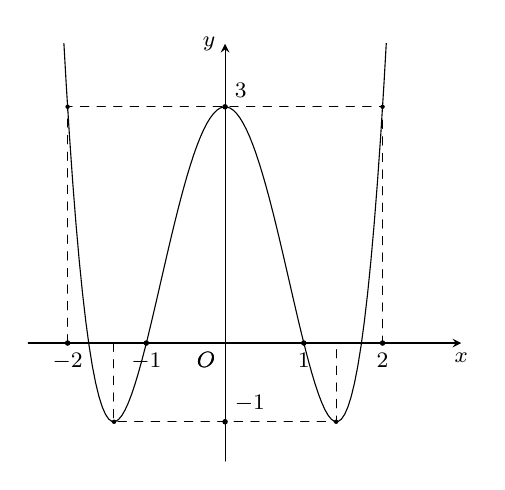
\begin{tikzpicture}[line join=round,line cap=round,>=stealth,scale=1,font=\footnotesize]
			\draw[->] (-2.5,0)--(3,0)node[below]{$x$};
			\draw[->] (0,-1.5)--(0,3.8)node[left]{$y$};
			\begin{scope}
				\clip(-2.5,3.8)rectangle(2.5,-1.5);
				\draw[samples=100,domain=-2.06:2.06] plot (\x,{(\x)^4-4*(\x)^2+3});
			\end{scope}
			\draw(0,0)node[below left]{$O$};
			\draw[dashed]
			(-2,0)--(-2,3)--(2,3)--(2,0)
			(-1.4142,0)--(-1.4142,-1)--(1.4142,-1)--(1.4142,0)
			(0,0)node[below left]{$O$}
			;
			\foreach \i in {-2,-1,1,2}{\fill
				(\i,0)circle(1pt)node[below]{$\i$};}
			\foreach \i in {-1,3}{\fill
				(0,\i)circle(1pt)node[above right]{$\i$};}
			\fill(-2,3)circle(0.8pt)
			(-1.41,-1)circle(0.8pt)
			(1.41,-1)circle(0.8pt)
			(2,3)circle(0.8pt)
			;
	\end{tikzpicture}}
	\loigiai{
		Dựa vào đồ thị, suy ra hàm số đồng biến trên khoảng $(-1;0)$.
	}
\end{ex}

\begin{ex}%[Đề thi thử Tốt Nghiệp THPT Lần 1, SGD Bình Phước, 2023]%[12-EX-6-2023, Võ Hoàng Nghĩa]%[2D1Y4-1]
	Đường tiệm cận ngang của đồ thị hàm số $y=\dfrac{x}{x^2-1}$ là
	\choice
	{$y=1$}
	{$x=1$}
	{$x=-1$}
	{\True $y=0$}
	\loigiai{
		Ta có $\lim\limits_{x\to\pm\infty}\dfrac{x}{x^2-1}=0$.\\ 
		Do đó, tiệm cận ngang của đồ thị hàm số $y=\dfrac{x}{x^2-1}$ là $y=0$.
	}
\end{ex}

\begin{ex}%[Đề thi thử Tốt Nghiệp THPT Lần 1, SGD Bình Phước, 2023]%[12-EX-6-2023, Võ Hoàng Nghĩa]%[2D3Y2-1]
	Nếu $\displaystyle\int\limits_{-1}^1f(x)\mathrm{\,d}x=2$ và $\displaystyle\int\limits_{-1}^1g(x)\mathrm{\,d}x=-7$ thì $\displaystyle\int\limits_{-1}^1\left[f(x)-\dfrac{1}{7}g(x)\right]\mathrm{d}x$ bằng
	\choice
	{$1$}
	{$-3$}
	{$-1$}
	{\True $3$}
	\loigiai{
		Ta có $\displaystyle\int\limits_{-1}^1\left[f(x)-\dfrac{1}{7}g(x)\right]\mathrm{d}x=\int\limits_{-1}^1 f(x)\mathrm{\,d}x-\dfrac{1}{7}\int\limits_{-1}^1g(x)\mathrm{\,d}x=2-\dfrac{1}{7}\cdot (-7)=3$.
	}
\end{ex}

\begin{ex}%[Đề thi thử Tốt Nghiệp THPT Lần 1, SGD Bình Phước, 2023]%[12-EX-6-2023, Võ Hoàng Nghĩa]%[2H3Y3-1]
	Trong không gian $Oxyz$, cho đường thẳng $d\colon\dfrac{x-2}{-1}=\dfrac{y-1}{2}=\dfrac{z+3}{1}$. Véc-tơ nào dưới đây là một véc-tơ chỉ phương của $d$?
	\choice
	{\True $\overrightarrow{u}_3=\left(-1;2;1\right)$}
	{$\overrightarrow{u}_4=\left(-1;2;-1\right)$}
	{$\overrightarrow{u}_1=\left(2;1;-3\right)$}
	{$\overrightarrow{u}_2=\left(-2;-1;3\right)$}
	\loigiai{
		Đường thẳng $d$ nhận véc-tơ $\overrightarrow{u}_3=\left(-1;2;1\right)$ là một véc-tơ chỉ phương.
	}
\end{ex}

\begin{ex}%[Đề thi thử Tốt Nghiệp THPT Lần 1, SGD Bình Phước, 2023]%[12-EX-6-2023, Võ Hoàng Nghĩa]%[2D1Y2-1]
	Số điểm cực trị của hàm số $y=(x-1)^2 (x-2)$ là
	\choice
	{\True $2$}
	{$1$}
	{$0$}
	{$3$}
	\loigiai{
		Ta có $y'=2\left(x-1\right)\left(x-2\right)+\left(x-1\right)^2=\left(x-1\right)\left(3x-5\right)$ đổi dấu khi qua các điểm $x=1$; $x=\dfrac{5}{3}$.\\
		Suy ra hàm số có $2$ cực trị.
	}
\end{ex}

\begin{ex}%[Đề thi thử Tốt Nghiệp THPT Lần 1, SGD Bình Phước, 2023]%[12-EX-6-2023, Võ Hoàng Nghĩa]%[2D1B2-2]
	\immini
	{Cho hàm số $y=f(x)$ có đồ thị của hàm số $y=f'(x)$ như hình vẽ bên. Điểm cực tiểu của hàm số là
		\choice
		{$x=0$}
		{$x=1$}
		{$x=-1$}
		{\True $x=2$}}
	{\begin{tikzpicture}[font=\footnotesize,line join=round, line cap=round, >=stealth,scale=1] 
			\draw[->] (-2,0)--(2.5,0)node[below]{$x$};
			\draw[->](0,-2.3)--(0,1)node[left]{$y$};
			\begin{scope}
				\clip (-2,1)rectangle(3,-2);
				\draw[shorten <=0.5cm,shorten >=0.5cm]
				(-1.5,1.5)..controls++(282.21:0.33) and++(221.5:0.81)..(-0.4,-0.2)
				..controls++(43.72:1.37) and ++(176.73:0.75)..(1.35,-2.01)
				..controls++(5.17:0.36) and++(262.08:2.83)
				..(2.21,1.5)
				;
			\end{scope}
			\foreach \i in {-1,1,2}{\fill (\i,0)circle(1pt)node[above]{$\i$};}
			\foreach \i in {-1}{\fill (0,\i)circle(1pt)node[left]{$\i$};}
			\fill (0,0) circle(1pt) node[above right]{$O$};
	\end{tikzpicture}}
	\loigiai{
		Bảng biến thiên của hàm số $y=f(x)$
		\begin{center}
			
\begin{tikzpicture}
				\tkzTabInit[lgt=1.2]{$x$/0.6,$f'(x)$/0.6,$f(x)$/2}{$-\infty$,$-1$,$0$,$2$,$+\infty$}
				\tkzTabLine{,+,0,-,0,-,0,+,}
				\tkzTabVar{-/$-\infty$,+/$f(-1)$,R,-/$f(2)$,+/$+\infty$}
				\tkzTabIma{2}{4}{3}{$f(0)$}
			\end{tikzpicture}
		\end{center}
		Dựa vào bảng biến thiên ta thấy hàm số $y=f(x)$ đạt cực tiểu tại $x=2$.
	}
\end{ex}

\begin{ex}%[Đề thi thử Tốt Nghiệp THPT Lần 1, SGD Bình Phước, 2023]%[12-EX-6-2023, Võ Hoàng Nghĩa]%[2H3B1-1]
	Trong không gian $Oxyz$, cho $A(3;0;0)$, $B(0;4;0)$. Chu vi của tam giác $OAB$ bằng
	\choice
	{$25$}
	{\True $12$}
	{$14$}
	{$7$}
	\loigiai{
		Ta có $OA=\sqrt{3^2+0^2+0^2}=3$; $OB=\sqrt{0^2+4^2+0^2}=4$; $AB=\sqrt{3^2+4^2+0^2}=5$.\\
		Vậy chu vi $\Delta OAB$ bằng $3+4+5=12$.
	}
\end{ex}

\begin{ex}%[Đề thi thử Tốt Nghiệp THPT Lần 1, SGD Bình Phước, 2023]%[12-EX-6-2023, Võ Hoàng Nghĩa]%[2D1B5-4]
	Đồ thị của hàm số $y=\dfrac{1-x}{x+1}$ cắt trục $Oy$ tại điểm có tọa độ là
	\choice
	{$(1;1)$}
	{$(1;0)$}
	{\True $(0;1)$}
	{$(0;-1)$}
	\loigiai{
		Đồ thị hàm số cắt trục tung tại điểm $A(0;y)\Rightarrow y=\dfrac{1-0}{0+1}=1\Rightarrow A\left(0;1\right)$.
	}
\end{ex}

\begin{ex}%[Đề thi thử Tốt Nghiệp THPT Lần 1, SGD Bình Phước, 2023]%[12-EX-6-2023, Võ Hoàng Nghĩa]%[2D3B3-3]
	Thể tích khối tròn xoay thu được khi quay hình phẳng $(H)$ giới hạn bởi các đường $y=\dfrac{1}{3}{x^3}-x^2$, $y=0$, $x=0$ và $x=3$ quanh trục $Ox$ là
	\choice
	{$\dfrac{71}{35}$}
	{\True $\dfrac{81\pi}{35}$}
	{$\dfrac{81}{35}$}
	{$\dfrac{71\pi}{35}$}
	\loigiai{
		Thể tích khối tròn xoay sinh ra khi quay hình phẳng $(H)$ quanh trục $Ox$ là
		$$V=\pi\displaystyle\int\limits_0^3\left(\dfrac{1}{3}{x^3}-x^2\right)^2\mathrm{\,d}x=\pi\displaystyle\int\limits_0^3\left(\dfrac{1}{9}{x^6}-\dfrac{2}{3}{x^5}+x^4\right)\mathrm{\,d}x=\dfrac{81\pi}{35}.$$
		Vậy thể tích khối tròn xoay cần tính là  $V=\dfrac{81\pi}{35}$.
	}
\end{ex}

\begin{ex}%[Đề thi thử Tốt Nghiệp THPT Lần 1, SGD Bình Phước, 2023]%[12-EX-6-2023, Võ Hoàng Nghĩa]%[2D4B2-2]
	Cho các số phức $z=-1+2i$, $w=3-i$. Phần ảo của số phức $z\overline{w}$ bằng
	\choice
	{\True $5$}
	{$5i$}
	{$7$}
	{$7i$}
	\loigiai{
		Ta có $z\overline{w}=(-1+2i)(3+i)=-5+5i$.\\ 
		Do đó phần ảo của số phức $z\overline{w}$ bằng $5$.
	}
\end{ex}

\begin{ex}%[Đề thi thử Tốt Nghiệp THPT Lần 1, SGD Bình Phước, 2023]%[12-EX-6-2023, Võ Hoàng Nghĩa]%[1D2B5-2]
	Một hộp đựng $9$ chiếc thẻ được đánh số từ $1$ đến $9$. Rút ngẫu nhiên ra hai thẻ rồi nhân hai số ghi trên hai thẻ lại với nhau. Xác suất để kết quả nhận được là một số chẵn bằng
	\choice
	{\True $\dfrac{13}{18}$}
	{$\dfrac{5}{18}$}
	{$\dfrac{1}{6}$}
	{$\dfrac{1}{2}$}
	\loigiai{
		Số phần tử không gian mẫu là $n\left(\Omega\right)=\mathrm{C}_9^2$.\\
		Gọi biến cố $A$: \lq\lq tích hai thẻ là một số chẵn\rq\rq.\\
		Ta có hai khả năng xảy ra $A$: hai thẻ lấy ra là đều chẵn hoặc hai thẻ lấy ra gồm $1$ chẵn và $1$ lẻ.\\
		Suy ra $n(A)=\mathrm{C}_4^2+4\cdot5$.\\
		Vậy xác suất cần tính là $\mathrm{P}(A)=\dfrac{\mathrm{C}_4^2+4\cdot 5}{\mathrm{C}_9^2}=\dfrac{13}{18}$.
	}
\end{ex}

\begin{ex}%[Đề thi thử Tốt Nghiệp THPT Lần 1, SGD Bình Phước, 2023]%[12-EX-6-2023, Võ Hoàng Nghĩa]%[2D3B1-1]
	Nếu $F(x)$ là một nguyên hàm của hàm số $f(x)=\dfrac{1}{\sqrt{x^2+1}}$ thì $F'\left(2\sqrt{2}\right)-F'(0)$ bằng
	\choice
	{\True $-\dfrac{2}{3}$}
	{$-\dfrac{8}{9}$}
	{$\dfrac{1}{3}$}
	{$\dfrac{2}{3}$}
	\loigiai{
		Do $F(x)$ là một nguyên hàm của hàm số $f(x)=\dfrac{1}{\sqrt{x^2+1}}$, nên $F'(x)=f(x)=\dfrac{1}{\sqrt{x^2+1}}$.\\
		Suy ra $F'\left(2\sqrt{2}\right)=\dfrac{1}{3}$ và $F'(0)=1$ $\Rightarrow{F}'\left(2\sqrt{2}\right)-F'(0)=-\dfrac{2}{3}$.
	}
\end{ex}

\begin{ex}%[Đề thi thử Tốt Nghiệp THPT Lần 1, SGD Bình Phước, 2023]%[12-EX-6-2023, Võ Hoàng Nghĩa]%[2H3B3-3]
	Trong không gian $Oxyz$, cho điểm $M\left(2;-6;3\right)$ và đường thẳng $d\colon\heva{
		& x=1+3t\\ 
		& y=-2-2t\\ 
		& z=t\\}$. Tọa độ hình chiếu vuông góc của $M$ lên $d$ là
	\choice
	{$\left(1;-2;0\right)$}
	{$\left(-8;4;-3\right)$}
	{$\left(1;2;1\right)$}
	{\True $\left(4;-4;1\right)$}
	\loigiai{
		Gọi $H$ là hình chiếu vuông góc của $M$ lên $d$.\\
		Suy ra $H\in d$ nên $H\left(1+3t;-2-2t;t\right)$. Suy ra $\overrightarrow{MH}=\left(3t-1;4-2t;t-3\right)$.\\
		Ta có $MH\perp d$ nên $\overrightarrow{MH}\cdot\overrightarrow{u}_d=0\Leftrightarrow 3\left(3t-1\right)-2\left(4-2t\right)+\left(t-3\right)=0\Leftrightarrow t=1$.\\
		Vậy $H\left(4;-4;1\right)$.
	}
\end{ex}

\begin{ex}%[Đề thi thử Tốt Nghiệp THPT Lần 1, SGD Bình Phước, 2023]%[12-EX-6-2023, Võ Hoàng Nghĩa]%[2D1B5-3]
	\immini
	{Cho hàm số bậc ba $y=f(x)$ có đồ thị như hình vẽ bên. Số giá trị nguyên của tham số $m$ để phương trình $f(x)+3m=0$ có ba nghiệm phân biệt là
		\choice
		{$3$}
		{$0$}
		{$2$}
		{\True $1$}}
	{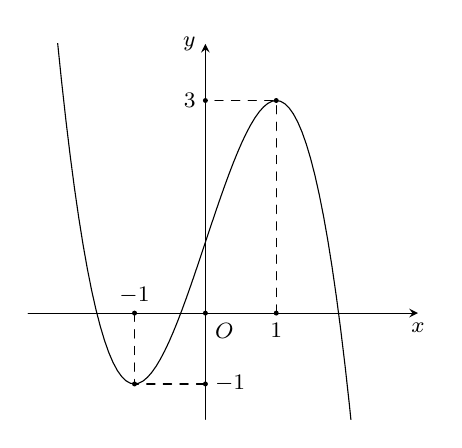
\begin{tikzpicture}[font=\footnotesize,line join=round, line cap=round, >=stealth,scale=0.9] 
			\draw[->] (-2.5,0)--(3,0)node[below]{$x$};
			\draw[->] (0,-1.5)--(0,3.8)node[left]{$y$};
			\begin{scope}
				\clip (-2.5,3.8)rectangle(3,-1.5);
				\draw[samples=100,domain=3:-3] plot (\x,{-(\x)^3+3*(\x)+1});
			\end{scope}
			\draw(0,0)node[below right]{$O$};
			\draw[dashed]
			(1,0)node[below]{$1$}
			(-1,0)node[above]{$-1$}
			(0,-1)node[right]{$-1$}
			(0,3)node[left]{$3$}
			(1,0)--(1,3)--(0,3)
			(-1,0)--(-1,-1)--(0,-1)
			;
			\foreach \i in {-1,1,0}{\fill
				(\i,0)circle(1pt);}
			\foreach \i in {-1,3}{\fill
				(0,\i)circle(1pt);}
\fill (-1,-1) circle(1pt) (1,3) circle(1pt); 
	\end{tikzpicture}}
	
	\loigiai{
		Số nghiệm của phương trình $f(x)+3m=0$ là số giao điểm của đồ thị hàm số $y=f(x)$ và đường thẳng $y=-3m$.\\
		Dựa vào đồ thị, phương trình $f(x)+3m=0$ có ba nghiệm phân biệt khi và chỉ khi $$-1<-3m<3\Leftrightarrow-1<m<\dfrac{1}{3}.$$
		Vì $m\in\mathbb{Z}$ nên $m=0$.
	}
\end{ex}

\begin{ex}%[Đề thi thử Tốt Nghiệp THPT Lần 1, SGD Bình Phước, 2023]%[12-EX-6-2023, Võ Hoàng Nghĩa]%[2D2B5-3]
	Tích tất cả các nghiệm của phương trình $\log_3^2 x-2\log_3 x-7=0$ là
	\choice
	{$1$}
	{$2$}
	{\True $9$}
	{$-7$}
	\loigiai{
		Đặt $\log_3x=t\Rightarrow x=3^t$.\\
		Phương trình $\log_3^2x-2\log_3^{}x-7=0$ $(1)$ trở thành $t^2-2t-7=0$. $(2)$\\
		Nhận thấy phương trình $(2)$ có $2$ nghiệm phân biệt $t_1$, $t_2$ và $t_1+t_2=2$\\
		Nên phương trình $(2)$ có đúng $2$ nghiệm $x_1$, $x_2$.\\
		Suy ra $x_1x_2=3^{t_1}{3^{t_2}}=3^{t_1+t_{^2}}=9$.
	}
\end{ex}

\begin{ex}%[Đề thi thử Tốt Nghiệp THPT Lần 1, SGD Bình Phước, 2023]%[12-EX-6-2023, Võ Hoàng Nghĩa]%[2D4K2-4]
	Xét các số phức $z$ thỏa mãn $\left(\overline{z}-2i\right)\left(z+2\right)$ là số thuần ảo. Trên mặt phẳng tọa độ, tập hợp tất cả các điểm biểu diễn các số phức $z$ là một đường tròn có bán kính bằng
	\choice
	{$4$}
	{$2\sqrt{2}$}
	{\True $\sqrt{2}$}
	{$2$}
	\loigiai{
		Gọi $z=a+bi$, $a,b\in\mathbb{R}$.\\
		Ta có $\left(\overline{z}-2i\right)\left(z+2\right)=\left(a-bi-2i\right)\left(a+bi+2\right)=a^2+2a+b^2+2b-2\left(a+b+2\right)i$.\\
		Vì $\left(\overline{z}-2i\right)\left(z+2\right)$ là số thuần ảo nên $a^2+2a+b^2+2b=0\Leftrightarrow{\left(a+1\right)^2}+\left(b+1\right)^2=2$.\\
		Trên mặt phẳng tọa độ, tập hợp tất cả các điểm biểu diễn các số phức $z$ là một đường tròn có bán kính bằng $\sqrt{2}$.
	}
\end{ex}

\begin{ex}%[Đề thi thử Tốt Nghiệp THPT Lần 1, SGD Bình Phước, 2023]%[12-EX-6-2023, Võ Hoàng Nghĩa]%[2D3K3-1]
	Cho hàm số $y=f(x)$ có đạo hàm liên tục trên $\mathbb{R}\setminus \{ 0\}$ thỏa mãn $xf'(x)+2x^2=f(x)+2x^3$, $\forall x\ne 0$ và $f(1)=2$. Diện tích hình phẳng giới hạn bởi các đường $y=f(x)$ và $y=f'(x)$ bằng
	\choice
	{$\dfrac{5}{4}$}
	{$\dfrac{5}{2}$}
	{$\dfrac{2}{3}$}
	{\True $\dfrac{4}{3}$}
	\loigiai{
		Ta có $xf'(x)+2x^2=f(x)+2x^3\Leftrightarrow\dfrac{xf'(x)-(x)' f(x)}{x^2}=2x-2\Leftrightarrow{\left(\dfrac{f(x)}{x}\right)'}=2x-2,\forall x\ne 0$.\\
		Do đó $\dfrac{f(x)}{x}=x^2-2x+C$, $f(1)=2\Rightarrow C=3\Rightarrow f(x)=x^3-2x^2+3x$.\\
		Suy ra $f'(x)=3x^2-4x+3$.\\
		Xét phương trình hoành độ giao điểm của $y=f(x)$ và $y=f'(x)$
		$$x^3-2x^2+3x=3x^2-4x+3\Leftrightarrow\hoac{
			& x=3\\ 
			& x=1.\\}$$\\ 
		Vậy diện tích phẳng giới hạn bởi các đường $y=f(x)$ và $y=f'(x)$ là $S=\displaystyle\int\limits_1^3\left|f(x)-f'(x)\right|\mathrm{\,d}x=\dfrac{4}{3}$.
	}
\end{ex}

\begin{ex}%[Đề thi thử Tốt Nghiệp THPT Lần 1, SGD Bình Phước, 2023]%[12-EX-6-2023, Võ Hoàng Nghĩa]%[2D2K5-5]
	Cho bất phương trình $2^{x^2+x}+2x\le 2^{3-x}-x^2+3$ có tập nghiệm là $[a;b]$. Giá trị của biểu thức $2a+b$ bằng
	\choice
	{$3$}
	{$-2$}
	{$1$}
	{\True $-5$}
	\loigiai{
		Ta có $2^{x^2+x}+2x\le{2^{3-x}}-x^2+3\Leftrightarrow{2^{x^2+x}}+x^2+x\le{2^{3-x}}+3-x$. $(1)$\\
		Xét hàm số $f(t)=2^t+t$, có $f'(t)=2^t\ln 2+1>0,\forall t\in\mathbb{R}$.\\
		Vậy hàm số $f(t)$ đồng biến trên $\mathbb{R}$. Do đó
		$$(1)\Leftrightarrow f\left(x^2+x\right)\le f\left(3-x\right)\Leftrightarrow{x^2}+x\le 3-x\Leftrightarrow-3\le x\le 1.$$
		Suy ra tập nghiệm của bất phương trình đã cho là $S=[-3;1]$.\\
		Vậy $a=-3$, $b=1\Rightarrow T=2a+b=-5$.
	}
\end{ex}

\begin{ex}%[Đề thi thử Tốt Nghiệp THPT Lần 1, SGD Bình Phước, 2023]%[12-EX-6-2023, Võ Hoàng Nghĩa]%[2H3K3-8]
	Trong không gian $Oxyz$, cho đường thẳng $d\colon\dfrac{x+2}{4}=\dfrac{y-1}{-4}=\dfrac{z+2}{3}$ và mặt phẳng $(P)\colon2x-y+2z+1=0$. Đường thẳng $\Delta $ đi qua $E\left(-2;1;-2\right)$, song song với $(P)$ đồng thời tạo với $d$ góc bé nhất. Biết rằng $\Delta$ có một véc-tơ chỉ phương $\overrightarrow{u}=\left(m;n;1\right).$ Tính $T=m^2-n^2$.
	\choice
	{$T=4$}
	{$T=3$}
	{\True $T=-4$}
	{$T=-5$}
	\loigiai{
		Mặt phẳng $(P)$ có véc-tơ pháp tuyến là $\overrightarrow{n}=\left(2;-1;2\right)$; đường thẳng $d$ có véc-tơ chỉ phương là $\overrightarrow{v}=\left(4;-4;3\right)$.\\
		Do $\Delta\parallel (P)$ nên $\overrightarrow{u}\perp\overrightarrow{n}\Leftrightarrow 2m-n+2=0\Leftrightarrow n=2m+2$.\\
		Mặt khác, ta có $\begin{aligned}[t]
			\cos{\left(\Delta ,d\right)}&=\dfrac{\left|\overrightarrow{u}\overrightarrow{v}\right|}{\left|\overrightarrow{u}\right|\left|\overrightarrow{v}\right|}=\dfrac{\left| 4m-4n+3\right|}{\sqrt{m^2+n^2+1}\sqrt{4^2+\left(-4\right)^2+3^2}}=\dfrac{\left| 4m+5\right|}{\sqrt{41\left(5m^2+8m+5\right)}}\\
			&=\dfrac{1}{\sqrt{41}}\sqrt{\dfrac{\left(4m+5\right)^2}{5m^2+8m+5}}=\dfrac{1}{\sqrt{41}}\sqrt{\dfrac{16m^2+40m+25}{5m^2+8m+5}}
		\end{aligned}$.\\
		Vì $0^\circ\le{\left(\Delta,d\right)}\le 90^\circ $ nên ${\left(\Delta,d\right)}$ bé nhất khi và chỉ khi $\cos{\left(\Delta,d\right)}$ lớn nhất\\
		Xét hàm số $f(t)=\dfrac{16t^2+40t+25}{5t^2+8t+5} \Rightarrow f'(t)=\dfrac{-72t^2-90t}{\left(5t^2+8t+5\right)^2}$.\\
		Bảng biến thiên
		\begin{center}
			
\begin{tikzpicture}
				\tkzTabInit[lgt=1,espcl=3]{$t$/0.7,$f'(t)$/0.7,$f(t)$/2.5}{$-\infty$,$-\tfrac{5}{4}$,$0$,$+\infty$}
				\tkzTabLine{,-,0,+,0,-,}
				\tkzTabVar{+/$\dfrac{16}{5}$,-/$0$,+/$5$,-/$\dfrac{16}{5}$}
			\end{tikzpicture}
		\end{center}
		Dựa vào bảng biến thiên ta có
		$\max\limits_{\mathbb{R}} f(t)=f(0)=5$.\\ 
		Suy ra $\left(\Delta,d\right)$ bé nhất khi $m=0\Rightarrow n=2$.\\
		Do đó $T=m^2-n^2=-4$.
	}
\end{ex}

\begin{ex}%[Đề thi thử Tốt Nghiệp THPT Lần 1, SGD Bình Phước, 2023]%[12-EX-6-2023, Võ Hoàng Nghĩa]%[2H1K3-4]
	Cho hình chóp tứ giác đều $S.ABCD$ có cạnh đáy bằng $a$, cạnh bên bằng $\dfrac{a\sqrt{5}}{2}$. Số đo góc giữa hai mặt phẳng $\left(SAB\right)$ và $\left(ABCD\right)$ là
	\choice
	{\True $60^\circ$}
	{$90^\circ$}
	{$45^\circ$}
	{$30^\circ$}
	\loigiai{
		\immini
		{Gọi $O$ là tâm của $ABCD$, $I$ là trung điểm của $AB$.\\ 
			Ta có $\heva{&AB\perp OI\\&AB\perp SO}\Rightarrow AB\perp (SIO)\Rightarrow AB\perp SI$.\\
			Ta có $\heva{&AB\perp OI,OI\subset(ABCD)\\&
				AB\perp SI,SI\subset (SAB)\\
				&(SAB)\cap(ABCD)=AB.\\}$\\
			Suy ra $\left((SAB),(ABCD)\right)=(SI,OI)=\widehat{SIO}$.\\
			Ta có $SI=\sqrt{S{A^2}-A{I^2}}=\sqrt{\left(\dfrac{a\sqrt{5}}{2}\right)^2-\left(\dfrac{a}{2}\right)^2}=a$.\\ 
			Suy ra $\cos\widehat{SIO}=\dfrac{OI}{SI}=\dfrac{\dfrac{a}{2}}{a}=\dfrac{1}{2}\Rightarrow\widehat{SIO}=60^\circ$.}
		{\begin{tikzpicture}[scale=1, font=\footnotesize, line join=round, line cap=round, >=stealth]
				\def\bc{4} % cạnh BC
				\def\ba{2} % cạnh BA
				\def\h{4} % đường cao
				\def\gocB{30} % góc B của đáy
				\coordinate[label=below left:$B$] (B) at (0,0);
				\coordinate[label=above right:$A$] (A) at (\gocB:\ba);
				\coordinate[label=below:$C$] (C) at (\bc,0);
				\coordinate[label=right:$D$] (D) at ($(C)-(B)+(A)$);
				\coordinate[label=below:$O$] (O) at ($(A)!.5!(C)$);
				\coordinate[label=above:$S$] (S) at ($(O)+(90:\h)$);
				\coordinate[label=left:$I$] (I) at ($(A)!0.5!(B)$);
				;
				\draw (B)--(C)--(D)--(S)--cycle (S)--(C);
				\draw[dashed] (C)--(A)--(D)--(B) (O)--(S)--(A)--(B) (S)--(I)--(O);
				\foreach \diem in {A,B,C,D,S,O,I}	\fill (\diem)circle(1.5pt);
			\end{tikzpicture}
		}
		
	}
\end{ex}

\begin{ex}%[Đề thi thử Tốt Nghiệp THPT Lần 1, SGD Bình Phước, 2023]%[12-EX-6-2023, Võ Hoàng Nghĩa]%[2D4K5-1]
	Cho các số phức $z$, $w$ thỏa mãn $\left|w-3+i\right|=3\sqrt{2}$ và $\dfrac{w}{z-2}=1+i$. Giá trị lớn nhất của biểu thức $P=\left|z-1-2i\right|+\left| z-5-2i\right|$ bằng
	\choice
	{\True $2\sqrt{53}$}
	{$\sqrt{52}+\sqrt{55}$}
	{$3+\sqrt{134}$}
	{$\dfrac{29}{2}$}
	\loigiai{
		Từ giả thiết $\dfrac{w}{z-2}=1+i$, ta có $w=\left(z-2\right)\left(1+i\right)$.\\ 
		Khi đó
		$\begin{aligned}[t]
			\left|w-3+i\right|=3\sqrt{2}&\Leftrightarrow\left|\left(z-2\right)\left(1+i\right)-3+i\right|=3\sqrt{2}\\
			&\Leftrightarrow\left|\left(1+i\right)\left(z-3+2i\right)\right|=3\sqrt{2}\\
			&\Leftrightarrow\left|z-3+2i\right|=3.
		\end{aligned}$\\
		Suy ra điểm $M\left(x;y\right)$ biểu diễn cho số phức $z$ sẽ thuộc đường tròn $(C)\colon\left(x-3\right)^2+\left(y+2\right)^2=9$.\\
		Ta có $P=MA+MB$, với $A\left(1;2\right)$, $B\left(5;2\right)$.
		\begin{center}
			\begin{tikzpicture}[font=\footnotesize,line join=round, line cap=round, >=stealth,scale=1]
				\draw[->] (-1.5,0)--(7,0)node[below]{$x$};
				\draw[->] (0,-6)--(0,3)node[left]{$y$};
				\draw(3,-2)circle(3cm);
				\foreach \i in {-1,1,2,...,6}{\fill (\i,0)circle(1pt)node[above]{$\i$};}
				\foreach \i in {-5,-4,...,-1,1,2}{\fill (0,\i)circle(1pt)node[left]{$\i$};}
				\path 
				(1,2) coordinate (A)
				++(0:4) coordinate (B)
				($(A)!0.5!(B)$) coordinate (H)
				++(-90:7) coordinate (K)
				(3,-2)coordinate (I)
				++(15:3) coordinate (M)
				;
				\path (0,0)node[below left]{$O$};
				\foreach \x/\y in {K/-90,M/0,A/90,B/90,H/90,I/-45}{\fill (\x) circle (0.8pt)++(\y:0.3)node{$\x$};}
				\draw (I)--(M) (A)--(B) (H)--(K) (A)--(M);
			\end{tikzpicture}
		\end{center}
		Gọi $H$ là trung điểm của $AB$, ta có $H\left(3;2\right)$.\\ 
		Khi đó $P=MA+MB\le\sqrt{2\left(MA^2+MB^2\right)}=\sqrt{4MH^2+AB^2}$.\\
		Mặt khác $MH\le KH$ với mọi điểm $M\in (C)$, nên $$P \le \sqrt{4KH^2+AB^2}=\sqrt{4\left(IH+R\right)^2+AB^2}=2\sqrt{53}.$$
		Vậy $P_{\max}=2\sqrt{53}$ khi $\heva{
			& M\equiv K\\ 
			& MA=MB\\}$ hay $z=3-5i$ và $w=6-4i$.
	}
\end{ex}

\begin{ex}%[Đề thi thử Tốt Nghiệp THPT Lần 1, SGD Bình Phước, 2023]%[12-EX-6-2023, Võ Hoàng Nghĩa]%[2H1K3-4]
	Cho hình chóp $S.ABCD$ có $SA$ vuông góc với mặt phẳng $ABCD$, đáy $ABCD$ là hình chữ nhật. Biết rằng $SA=a$, $AB=a$, $AD=2a$. Tính theo $a$ khoảng cách từ điểm $C$ đến mặt phẳng $\left(SBD\right)$.
	\choice
	{$\dfrac{4a}{3}$}
	{\True $\dfrac{2a}{3}$}
	{$\dfrac{a}{2}$}
	{$\dfrac{a}{3}$}
	\loigiai{
		\begin{center}
			\begin{tikzpicture}[scale=1, font=\footnotesize, line join=round, line cap=round, >=stealth]
				\def\bc{5} % cạnh BC
				\def\ba{2.4} % cạnh BA
				\def\h{4} % đường cao
				\def\gocB{40} % góc B của đáy
				\coordinate[label=below left:$B$] (B) at (0,0);
				\coordinate[label=above left:$A$] (A) at (\gocB:\ba);
				\coordinate[label=below:$C$] (C) at (\bc,0);
				\coordinate[label=right:$D$] (D) at ($(C)-(B)+(A)$);
				\coordinate[label=above:$S$] (S) at ($(A)+(90:\h)$);
				\draw (B)--(C)--(D)--(S)--cycle (S)--(C);
				\draw[dashed] (A)--(D) (S)--(A)--(B);
				\foreach \diem in {A,B,C,D,S}	\fill (\diem)circle(1.5pt);
				\path 
				(intersection of B--D and A--C) coordinate (O)
				(barycentric cs:B=1.8,D=1.2) coordinate (H)
				(barycentric cs:H=2,S=1) coordinate (K)
				;
				\draw[dashed] (B)--(D) (A)--(C) (A)--(H)--(S) (A)--(K);
				\foreach \x/\y in {O/-90,H/-90,K/0}{\fill (\x) circle (0.8pt)++(\y:0.3)node{$\x$};}
				\foreach \x/\y/\z in {	S/A/D,S/A/B,A/H/B,A/K/H}{
					\draw
					pic[draw,angle radius=2mm]{right angle=\x--\y--\z};}
			\end{tikzpicture}
			
		\end{center}
		Gọi $O$ là tâm của hình chữ nhật $ABCD\Rightarrow \mathrm{d}(C,(SAB))=\mathrm{d}\left(A,\left(SBD\right)\right)$.\\
		Gọi $H$ là hình chiếu của $A$ lên $BD\Rightarrow AH\perp BD$ .\\
		Vì $\heva{& SA\perp\left(ABCD\right)\\ 
			& BD\subset\left(ABCD\right)\\ }\Rightarrow SA\perp BD$.\\
		Khi đó $\heva{& AH\perp BD\\ 
			& SA\perp BD\\ }\Rightarrow BD\perp\left(SAH\right)$.\\
		Trong $\left(SAH\right)$, gọi $K$ là hình chiếu của $A$ lên $SH\Rightarrow AK\perp SH$. $(1)$\\
		Mà $\heva{& BD\perp\left(SAH\right)\\ 
			& AK\subset\left(SAH\right)\\ }\Rightarrow BD\perp AK$. $(2)$\\
		Từ $(1)$ và $(2)$ suy ra $AK\perp\left(SBD\right)\Rightarrow AK=\mathrm{d}\left(A,\left(SBD\right)\right)$.\\
		$AH=\dfrac{2S_{\Delta ABD}}{BD}=\dfrac{2\cdot\tfrac{1}{2}\cdot AB\cdot AD}{\sqrt{A{B^2}+A{D^2}}}=\dfrac{2a^2}{\sqrt{a^2+4a^2}}=\dfrac{2a}{\sqrt{5}}$.\\ Suy ra $AK=\dfrac{AH\cdot SA}{\sqrt{AH^2+SA^2}}=\dfrac{\tfrac{2a}{\sqrt{5}}\cdot a}{\sqrt{\tfrac{4a^2}{5}+a^2}}=\dfrac{2a}{3}$ .\\
		Vậy $\mathrm{d}(C,(SAB))=\dfrac{2a}{3}$ .
	}
\end{ex}

\begin{ex}%[Đề thi thử Tốt Nghiệp THPT Lần 1, SGD Bình Phước, 2023]%[12-EX-6-2023, Võ Hoàng Nghĩa]%[2H1K3-2]
	Cho hình lăng trụ $ABC.A'B'C'$ có các mặt bên đều là hình vuông. Gọi $M$, $N$ lần lượt là trung điểm của các cạnh $BC$, $A'C'$. Biết khoảng cách giữa hai đường thẳng $MN$ và $AB'$ bằng $\dfrac{a\sqrt{3}}{2}$. Thể tích khối chóp $A'.ABC$ bằng
	\choice
	{$a^3\sqrt{3}$}
	{$\dfrac{a^3\sqrt{3}}{3}$}
	{$2a^3\sqrt{3}$}
	{\True $\dfrac{2a^3\sqrt{3}}{3}$}
	\loigiai{
		\begin{center}
			\begin{tikzpicture}[scale=1, font=\footnotesize, line join=round, line cap=round, >=stealth]
				\def\ac{4} % cạnh AC
				\def\ab{2} % cạnh AB
				\def\h{4} % chiều cao
				\def\gocA{50} % góc A của đáy
				\coordinate[label=left:$A$] (A) at (0,0);
				\coordinate[label=right:$C$] (C) at (\ac,0);
				\coordinate[label=below left:$B$] (B) at (-\gocA:\ab);
				\coordinate[label=left:$A'$] (A') at ($(A)+(90:\h)$);
				\coordinate[label=below left:$B'$] (B') at ($(B)-(A)+(A')$);
				\coordinate[label=right:$C'$] (C') at ($(C)-(A)+(A')$);
				\draw (A')--(A)--(B)--(C)--(C')--(A')--(B')--(C') (B)--(B');
				\draw[dashed] (A)--(C);
				\foreach \diem in {A,B,C,A',B',C'} \fill (\diem)circle(1.5pt);
				\path 
				($(B)!0.5!(C)$) coordinate (M)
				($(A')!0.5!(C')$) coordinate (N)
				($(B')!0.5!(C')$) coordinate (K)
				($(A)!0.5!(B)$) coordinate (I)
				($(B)!0.5!(I)$) coordinate (J)
				;
				\foreach \x/\y in {M/-90,N/90,K/-15,I/180,J/180}{\fill (\x) circle (0.8pt)++(\y:0.3)node{$\x$};}
				\draw  (N)--(K)--(M) (B')--(A)
				;
				\draw[dashed] (C)--(I) (M)--(J)(N)--(M) ;
			\end{tikzpicture}
			
		\end{center}
		Từ giả thiết ta có $ABC.A'B'C'$ là lăng trụ đứng và có hai mặt đáy là các tam giác đều.\\
		Gọi $K$ là trung điểm của $B'C'$ ta có $MK\parallel BB'$ và $NK\parallel A'B'$ nên hai mặt phẳng $\left(MNK\right)$ và $\left(ABB'A'\right)$ song song. \\
		Suy ra khoảng cách giữa hai đường thẳng $MN$ và $AB'$ chính là khoảng cách giữa hai mặt phẳng $\left(MNK\right)$ và $\left(ABB'A'\right)$.\\
		Gọi $I$ là trung điểm của $AB$, gọi $J$ là trung điểm của $BI$. Khi đó, $MI\parallel CI$.\\ 
		Do tam giác $ABC$ đều và lăng trụ đã cho đứng nên $CI\perp\left(ABB'A'\right)$ $\Rightarrow MJ\perp\left(ABB'A'\right)$.\\
		Suy ra $ \mathrm{d}\left(\left(MNK\right),\left(ABB'A'\right)\right)=MJ$.\\ Suy ra $\mathrm{d}\left(M,\left(ABB'A'\right)\right)=MJ\Rightarrow MJ=\dfrac{a\sqrt{3}}{2}\Rightarrow CI=2MJ=a\sqrt{3}\Rightarrow AB=2a.$\\
		Ta có $V_{A'.ABC}=\dfrac{1}{3}AA'\cdot S_{ABC}=\dfrac{1}{3}\cdot 2a\cdot\dfrac{4a^2\sqrt{3}}{4}=\dfrac{2a^3\sqrt{3}}{3}$.
	}
\end{ex}

\begin{ex}%[Đề thi thử Tốt Nghiệp THPT Lần 1, SGD Bình Phước, 2023]%[12-EX-6-2023, Võ Hoàng Nghĩa]%[2H2K1-1]
	Cho khối nón đỉnh $S$ và tâm của đường tròn đáy là $O$. Gọi $M$, $N$ là hai điểm thuộc đường tròn đáy sao cho $\tan\widehat{SMO}=\dfrac{4}{3}$; $\widehat{MSN}=60^\circ$ và khoảng cách từ $O$ đến mặt phẳng $(SMN)$ bằng $\dfrac{\sqrt{22}}{5}$. Thể tích của khối nón đã cho bằng
	\choice
	{\True $\dfrac{9\pi\sqrt{6}}{8}$}
	{$\dfrac{45\pi\sqrt{6}}{8}$}
	{$\dfrac{15\pi\sqrt{6}}{8}$}
	{$\dfrac{27\pi\sqrt{6}}{8}$}
	\loigiai{
		\begin{center}
			\begin{tikzpicture}[font=\footnotesize,line join=round, line cap=round, >=stealth,scale=1.5] 
				\def\a{2};\def\b{0.4};\def\h{4};
				%Gán tọa độ.
				\coordinate (O) at (0,0);
				\coordinate (S) at ($(O)+(0,\h)$);
				\coordinate (A) at ($(O)-(\a,0)$);
				\coordinate (B) at ($(O)+(\a,0)$);
				%Vẽ khối nón.
				\draw (A) arc (-180:0:\a cm and \b cm) (A)--(S)--(B);
				\draw[dashed] (S)--(O) (A)--(B) (A) arc (180:0:\a cm and \b cm);
				\path 
				(A)arc(-180:-140:\a cm and \b cm) coordinate (M)
				(A)arc(-180:-250:\a cm and \b cm) coordinate (N)
				;
				\draw[dashed] (M)--(N) (S)--(N);
				\draw (S)--(M);
				\path 
				(barycentric cs:M=1,N=2) coordinate (I)
				(barycentric cs:S=1,I=3) coordinate (H)
				;
				\draw[dashed](S)--(I) (O)--(H)(O)--(I);
				%Gọi tên điểm.
				\foreach \x/\y in {S/90,O/-90,A/180,B/0,M/-90,N/-70,H/180,I/180}{\fill (\x) circle (1pt) ($(\x)+(\y:0.15cm)$) node{$\x$};}
			\end{tikzpicture}
		\end{center}
		Gọi $I$ là trung điểm của $MN$, $H$ là hình chiếu của $O$ trên $SI$ ta có $OH\perp\left(SMN\right)$.\\
		Suy ra $OH$ chính là khoảng cách từ $O$ đến $(SMN)$ $\Rightarrow OH=\dfrac{\sqrt{22}}{5}$.\\
		Đặt $SO=x$. Ta có $\tan\widehat{SMO}=\dfrac{4}{3}\Rightarrow\dfrac{OS}{OM}=\dfrac{4}{3}\Rightarrow OM=\dfrac{3OS}{4}=\dfrac{3x}{4}$.\\
		Khi đó $SM=\sqrt{O{S^2}+O{M^2}}=\sqrt{x^2+\dfrac{9x^2}{16}}=\dfrac{5x}{4}$.\\
		Do $SM=SN$, $\widehat{MSN}=60^\circ$.\\
		Suy ra $\triangle SMN$ đều $\Rightarrow SI=\dfrac{SM\sqrt{3}}{2}=\dfrac{\dfrac{5x}{4}.\sqrt{3}}{2}=\dfrac{5x\sqrt{3}}{8}$.\\
		Và $OI=\sqrt{S{I^2}-O{S^2}}=\sqrt{\dfrac{75x^2}{64}-x^2}=\dfrac{x\sqrt{11}}{8}$ .\\
		Ta có $OH\cdot SI=OS\cdot OI\Rightarrow\dfrac{\sqrt{22}}{5}\cdot\dfrac{5x\sqrt{3}}{8}=x\cdot\dfrac{x\sqrt{11}}{8}\Rightarrow\sqrt{22}\cdot\sqrt{3}=x\sqrt{11}$.\\
		Suy ra $ x=\sqrt{6}\Rightarrow OM=\dfrac{3\sqrt{6}}{4}$.\\
		Khi đó thể tích khối nón là $V=\dfrac{1}{3}SO\cdot\pi\cdot O{M^2}=\dfrac{1}{3}\cdot\sqrt{6}\cdot\pi \cdot\left(\dfrac{3\sqrt{6}}{4}\right)^2=\dfrac{54\pi\sqrt{6}}{48}=\dfrac{9\pi\sqrt{6}}{8}$.
	}
\end{ex}

\begin{ex}%[Đề thi thử Tốt Nghiệp THPT Lần 1, SGD Bình Phước, 2023]%[12-EX-6-2023, Võ Hoàng Nghĩa]%[2D3G2-2]
	Cho hàm số $f(x)$ liên tục trên $\mathbb{R}$. Gọi $F(x)$, $G(x)$ là hai nguyên hàm của $f(x)$ trên $\mathbb{R}$ thỏa mãn $F(4)-2G(4)=6$ và $F\left(-8\right)-2G\left(-8\right)=-2$. Khi đó $\displaystyle\int\limits_{-1}^3f\left(3x-5\right)\mathrm{\,d}x$ bằng
	\choice
	{$8$}
	{$\dfrac{8}{3}$}
	{$-3$}
	{\True $-\dfrac{8}{3}$}
	\loigiai{
		Ta có $G(x)=F(x)+C$.\\
		Theo đề bài $\heva{
			& F(4)-2G(4)=6\\ 
			&F(-8)-2G(-8)=-2\\}\Rightarrow\heva{
			&-F(4)-2C=6\\ 
			&-F(-8)-2C=-2\\}\Rightarrow F(4)-F(-8)=-8$.\\
		Vậy $\displaystyle\int\limits_{-1}^3f\left(3x-5\right)\mathrm{\,d}x=\dfrac{1}{3}\displaystyle\int\limits_{-8}^4f(x)\mathrm{\,d}x=\dfrac{1}{3}\left(F(4)-F(0)\right)=-\dfrac{8}{3}$.          
		
	}
\end{ex}

\begin{ex}%[Đề thi thử Tốt Nghiệp THPT Lần 1, SGD Bình Phước, 2023]%[12-EX-6-2023, Võ Hoàng Nghĩa]%[2D1G2-4]
	Cho hàm số $y=x^3+2(m-2t)x^2-5x+1$. Tìm tất cả các giá trị thực của tham số $m$ sao cho hàm số có hai điểm cực trị $x_1$, $x_2$ $\left(x_1<x_2\right)$ thỏa mãn $\left|x_1\right|-\left|x_2\right|=-2$.
	\choice
	{$\dfrac{7}{2}$}
	{$-1$}
	{\True $\dfrac{1}{2}$}
	{$5$}
	\loigiai{
		Ta có $y'=3x^2+4\left(m-2\right)x-5$.\\
		Khi đó $\Delta'=4\left(m-2\right)^2+15>0$ nên hàm số luôn có hai điểm cực trị $x_1$, $x_2$ $\left(x_1<x_2\right)$.\\
		Nhận xét $ac<0$ nên $x_1<0<x_2$.\\
		Suy ra $\left|x_1\right|-\left|x_2\right|=-2$ $\Leftrightarrow-x_1-x_2=-2$ $\Leftrightarrow\dfrac{b}{a}=-2$ $\Leftrightarrow\dfrac{4\left(m-2\right)}{3}=-2$ $\Leftrightarrow m=\dfrac{1}{2}$.
	}
\end{ex}

\begin{ex}%[Đề thi thử Tốt Nghiệp THPT Lần 1, SGD Bình Phước, 2023]%[12-EX-6-2023, Võ Hoàng Nghĩa]%[2D2G6-5]
	Có bao nhiêu số nguyên $x\in (0;2025)$ sao cho ứng với mỗi $x$, tồn tại ít nhất $10$ số nguyên $y\in\left(-3;10\right)$ thỏa mãn $2^y 3^x+6560\le 3^{2x^2+y}$?
	\choice
	{$2024$}
	{$2021$}
	{\True $2022$}
	{$2023$}
	\loigiai{
		Ta có $2^y{3^x}+6560\le{3^{2x^2+y}}\Leftrightarrow{\left(\dfrac{2}{3}\right)^y}{3^x}+6560\left(\dfrac{1}{3}\right)^y-3^{2x^2}\le 0$.\\
		Đặt $f(y)=\left(\dfrac{2}{3}\right)^y{3^x}+6560\left(\dfrac{1}{3}\right)^y-3^{2x^2}$.\\
		Bất phương trình trên có dạng $f(y)\le 0$, $y\in\left(-3;10\right)$.\\
		Ta có $f'(y)=\ln\left(\dfrac{2}{3}\right).\left(\dfrac{2}{3}\right)^y{3^x}+6560\left(\dfrac{1}{3}\right)^y\ln\left(\dfrac{1}{3}\right)<0$, $\forall y\in\left(-3;10\right)$.\\
		Do đó $f(y)$ nghịch biến trên $\left(-3;10\right)$.\\
		Khi đó $f\left(-2\right)>f\left(-1\right)>f(0)>f(1)>\cdots>f(9)$.\\
		Tồn tại ít nhất $10$ giá trị $y$ nguyên thuộc $\left(-3;10\right)$ thỏa mãn $f(y)\le 0$ khi và chỉ khi $f(0)\le 0\Leftrightarrow $ $3^x+6560\le{3^{2x^2}}$.\\ 
		Có $x$ nguyên, $x\in\left(0;2025\right)$ nên $x\ge 1$.\\
		Suy ra $6563\le{3^x}+6560\le{3^{2x^2}}\Leftrightarrow\hoac{
			&x\ge\sqrt{\dfrac{1}{2}{\log_3}6563}>2\\ 
			&x\le-\sqrt{\dfrac{1}{2}{\log_3}6563}<-2.\\}$\\
		Vậy $x\in\left\{3;4;5;\ldots;2024\right\}$ nên có $2022$ số nguyên $x$ thỏa yêu cầu bài toán.
	}
\end{ex}

\begin{ex}%[Đề thi thử Tốt Nghiệp THPT Lần 1, SGD Bình Phước, 2023]%[12-EX-6-2023, Võ Hoàng Nghĩa]%[2D4G4-1]
	Trên tập các số phức, xét phương trình $z^2-mz+m+8=0$ ($m$ là tham số thực). Có bao nhiêu giá trị nguyên của tham số $m$ để phương trình có hai nghiệm $z_1$, $z_2$ phân biệt thỏa mãn $\left|z_1\left(z_1^2+m{z_2}\right)\right|=\left(m^2-m-8\right)\left|z_2\right|$ ?
	\choice
	{$12$}
	{$6$}
	{\True $5$}
	{$11$}
	\loigiai{
		Xét phương trình $z^2-mz+m+8=0$, ta có $\Delta=m^2-4m-32$.
		\begin{itemize}
			\item Trường hợp 1: Xét $\Delta >0\Leftrightarrow{m^2}-4m-32>0\Leftrightarrow\hoac{
				& m>8\\ 
				& m<-4.\\}$\\ 
			Khi đó phương trình có hai nghiệm thực phân biệt.\\ 
			Ta có $z_1^2=m{z_1}-m-8$ suy ra $z_1^2+m{z_2}=m\left(z_1+z_2\right)-m-8=m^2-m-8$.\\ 
			Do đó $\left|z_1\left(z_1^2+m{z_2}\right)\right|=\left(m^2-m-8\right)\left|z_2\right|$ $\Leftrightarrow\left|m^2-m-8\right|\left|z_1\right|=\left(m^2-m-8\right)\left|z_2\right|$. $(*)$\\
			Nếu $z_1z_2=0$ thì $m+8=0\Rightarrow m=-8$ không thỏa mãn.\\ 
			Khi đó $(*)\Leftrightarrow\heva{
				&{m^2}-m-8>0\\ 
				&\left|z_1\right|=\left|z_2\right|\\ }\Leftrightarrow\heva{
				&{m^2}-m-8>0\\ 
				&{z_1}=-z_2\\}\Leftrightarrow\heva{
				&{m^2}-m-8>0\\ 
				& m=0\\}\Leftrightarrow m\in\varnothing$.
			\item Trường hợp 2: Xét $\Delta <0\Leftrightarrow-4<m<8$.\\ 
			Khi đó, phương trình có hai nghiệm phức phân biệt và $\left|z_1\right|=\left|z_2\right|$.\\
			Ta có $\begin{aligned}[t]
				\left|z_1\left(z_1^2+m{z_2}\right)\right|=\left(m^2-m-8\right)\left|z_2\right|&
				\Leftrightarrow\left|m^2-m-8\right|\left|z_1\right|=\left(m^2-m-8\right)\left|z_2\right|\\
				&\Leftrightarrow{m^2}-m-8\ge 0\\
				&\Leftrightarrow\hoac{
					& m\ge\dfrac{1+\sqrt{33}}{2}\\ 
					& m\le\dfrac{1-\sqrt{33}}{2}.\\}
			\end{aligned}$\\
			Kết hợp điều kiện ta được $m\in\left\{-3;4;5;6;7\right\}$.
		\end{itemize}
		Vậy có tất cả là $5$ số nguyên của tham số $m$.
	}
\end{ex}

\begin{ex}%[Đề thi thử Tốt Nghiệp THPT Lần 1, SGD Bình Phước, 2023]%[12-EX-6-2023, Võ Hoàng Nghĩa]%[2D1G1-3]
	Cho hàm số $y=f(x)$ liên tục trên $\mathbb{R}$ và có đạo hàm $f'(x)=x{\left(x-1\right)^2}\left(x^2+mx+16\right)$. Có bao nhiêu giá trị nguyên của tham số $m\in\left[-10;10\right]$ để hàm số $g(x)=f(x)+\dfrac{1}{4}{x^4}-\dfrac{2}{3}{x^3}+\dfrac{1}{2}{x^2}+2023$ đồng biến trên khoảng $\left(5;+\infty\right)$?
	\choice
	{$11$}
	{\True $19$}
	{$18$}
	{$10$}
	\loigiai{
		Ta có $\begin{aligned}[t]
			g'(x)&=f'(x)+x^3-2x^2+x\\
			&=x{\left(x-1\right)^2}\left(x^2+mx+16\right)+x{\left(x-1\right)^2}\\
			&=x{\left(x-1\right)^2}\left(x^2+mx+17\right).
		\end{aligned}$\\
		Hàm số $g(x)$ đồng biến trên khoảng $\left(5;+\infty\right)$ thì $g'(x)\ge 0,\forall x\in\left(5;+\infty\right)$.\\
		Suy ra $ x{\left(x-1\right)^2}\left(x^2+mx+17\right)\ge 0,\forall x>5\Leftrightarrow{x^2}+mx+17\ge 0,\forall x>5\Leftrightarrow m\ge\dfrac{-x^2-17}{x},\forall x>5$.\\
		Xét hàm số $h(x)=\dfrac{-x^2-17}{x}=-x-\dfrac{17}{x}$ trên khoảng $\left(5;+\infty\right)$\\
		Ta có $h'(x)=0\Leftrightarrow -1+\dfrac{17}{x^2}=0\Leftrightarrow x=\pm\sqrt{17}\notin(5;+\infty)\Rightarrow h'(x)<0,\forall x\in(5;+\infty)$.\\
		Suy ra $m\ge h(5)=-\dfrac{42}{5}$. \\
Kết hợp điều kiện $m$ nguyên và $m\in[-10;10]$, ta có $m\left\{-8;-7;\ldots;10\right\}$.\\
		Vậy có tất cả $19$ giá trị của $m$ thỏa mãn bài toán.
	}
\end{ex}

\begin{ex}%[Đề thi thử Tốt Nghiệp THPT Lần 1, SGD Bình Phước, 2023]%[12-EX-6-2023, Võ Hoàng Nghĩa]%[2H3G3-3]
	Trong không gian $Oxyz,$ cho hai điểm $A\left(0;0;-3\right)$, $B\left(2;0;-1\right)$ và mặt phẳng $(P)\colon3x-8y+7z-1=0$. Gọi $C\left(a;b;c\right)$ là điểm có tọa độ nguyên thuộc $(P)$ sao cho tam giác $ABC$ đều. Tổng $a+b+c$ bằng
	\choice
	{$7$}
	{\True $-3$}
	{$3$}
	{$-7$}
	\loigiai{
		Mặt phẳng trung trực $(\alpha)$ của đoạn thẳng $AB$ có phương trình là $\left(\alpha\right)\colon x+z+1=0$.\\
		Điểm $C$ thỏa mãn bài toán thuộc $\left(\alpha\right)$.\\ 
		Suy ra $C$ thuộc giao tuyến của $\left(\alpha\right)$ và $(P)$.\\
		Giao tuyến $\Delta $ thỏa mãn hệ phương trình $\heva{
			& 3x-8y+7z-1=0\\ 
			& x+z+1=0\\}\Rightarrow\Delta\colon\heva{
			& x=2t\\ 
			& y=-1-t\\ 
			& z=-1-2t.\\}$\\
		Điểm $C\in\Delta\Rightarrow C\left(2t;-1-t;-1-2t\right)$.\\
		Ta có $\heva{
			& CA=AB\\ 
			& CB=AB\\}$ mà $AB=2\sqrt{2}$.\\
		Suy ra ${\left(2t\right)^2}+\left(-1-t\right)^2+\left(2-2t\right)^2=8\Leftrightarrow 9t^2-6t-3=0\Leftrightarrow\hoac{
			&t=1\\ 
			&t=-\dfrac{1}{2}.}$
\begin{itemize}
\item Với $t=1$ suy ra $C(2;-2;-3)$.
\item Với $t=-\dfrac{1}{2}$ suy ra $C\left(-\dfrac{2}{2};-\dfrac{2}{2};-\dfrac{1}{3}\right)$.
\end{itemize}
	Vì $C$ là điểm có tọa độ nguyên nên ta chọn $C(2;-2;-3)$.\\
Suy ra $a=2$, $b=-2$ và $c=-3$. Vậy $a+b+c=-3$.
	}
\end{ex}

\Closesolutionfile{ans}
\begin{indapan}{10}
	{ans/ans-2-TT-23-SoGDDT-BinhPhuoc-23}
\end{indapan}
